\documentclass[a4paper,12pt, english]{article}
\usepackage[T1]{fontenc}
\usepackage[utf8]{inputenc}
\usepackage{graphicx}
\usepackage{babel}
\usepackage{amsmath}
\usepackage{ulem}
\usepackage{a4wide}
\usepackage{graphicx}
\usepackage{listings}
\usepackage{tabularx}
\usepackage{tabulary}
\usepackage{hyperref}

\begin{document}

\begin{titlepage}
\begin{center}
\textsc{\Large Machine Learning}\\[0.2cm]
\textsc{FYS-STK 4155}\\[1.0cm]
\textsc{\Large Project 1}\\[0.2cm]
\textsc{Kari Eriksen}\\[1.0cm]

\begin{abstract}
Here is my abstract going to be
\end{abstract}

\end{center}
\end{titlepage}

\section*{Introduction}

One of the simples models within the field of machine learning and statistical learning is linear regression. Because of its simplicity and the fact that it forms the base of many other more advanced methods it is highly recommended to understand it. \\ 
In this project we are studying several linear regression methods, the ordinary least square, Ridge regression and last the Lasso regression. Our first approach to understand these methods is to test them on the Franke function \ref{eq:frank}, a two-dimensional function which is widely used on testing interpolation and fitting algorithms. 
We evaluate our models abillity to predict the outcome(solution) using a resampling method called bootstrap and explore statistical errors such as bias, variance and Mean Square Error (MSE). All methods are explained in the sections below. \\
At last we will be using real data from a website that provides terrain data over the earth, \href{https://earthexplorer.usgs.gov/}{https://earthexplorer.usgs.gov/}, and test out method on these. 

 

\section*{Theory}

\begin{figure}
\centering
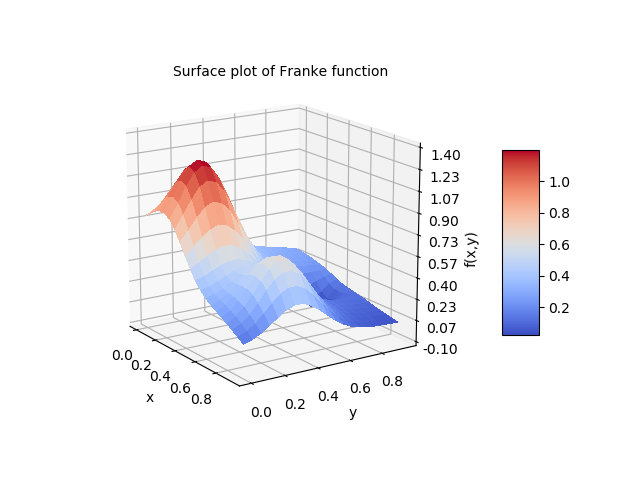
\includegraphics[width=1.0\textwidth]{/home/kari/Machine-Learning/Figures/franke.png}
\caption{Surface plot of Franke function for $x, y \in [0,1]$ generated with python code given in the assigment paper.}
\label{fig:franke}
\end{figure}


The Franke function is a two-dimensional function consisting of a sum of four exponatials, eq. \ref{eq:frank}. This will be the function which we will generate data from to feed our regression models. We define it for $x, y \in [0,1]$. \\
It can be seen represented as a surface plot in figure \ref{fig:franke}.

\begin{align}
f(x,y) &= \frac{3}{4}\exp{\left(-\frac{(9x-2)^2}{4} - \frac{(9y-2)^2}{4}\right)}+\frac{3}{4}\exp{\left(-\frac{(9x+1)^2}{49}- \frac{(9y+1)}{10}\right)} \nonumber \\
&+\frac{1}{2}\exp{\left(-\frac{(9x-7)^2}{4} - \frac{(9y-3)^2}{4}\right)} -\frac{1}{5}\exp{\left(-(9x-4)^2 - (9y-7)^2\right) } \label{eq:frank}
\end{align}




\section*{Regression methods}

\subsection*{Linear Regression}

Linear regression is a method in statistics that predicts the response of one or several explanatory variables. It assumes a linear relationship between the dependent and independent variables. At its simplest form we could try to find the stright line between two points. This equation is fairly simple.

\begin{equation}
\hat{y} = \hat{\beta_{0}} + \hat{\beta_{1}}x + \hat{\epsilon}
\end{equation}

Here $\hat{y}$ is a dependent variable, the outcome, $x$ is an independent variable, or the predictor, and $\hat{\beta_{0}}$ and $\hat{\beta_{1}}$ the intercept and slope respectively. $\epsilon$ is the error in our prediction. The solution for $\hat{\beta_{0}}$ and $\hat{\beta_{1}}$ in this problem is best found with least square and is also fairly easy. Calculating the mean over both variables $(\bar{x}$ and $\bar{y})$ we can find the parameters that give the prediction that differs the least from the exact solution.

\begin{equation}
\beta_1 = \frac{\sum^n (x_i - \bar{x})(y_i - \bar{y})}{\sum^n (x_i - \bar{x})^2}
\end{equation}

\begin{equation}
\beta_0 = \bar{y} - \beta_1 \bar{x}
\end{equation}

If we have several predictors we can extend our problem to a more general case.

\begin{equation}
\hat{y} = f(X) = \beta_{0} + \sum_{j=1}^{p} X_{j} \beta_{j}
\end{equation}

Now $X$ is a vector containing all predictors, $X^{\top} = \{X_0, X_1, X_2, X_3,..., X_p\}$, $\beta_0$ is the intercept and $\beta_j$ is a vector keeping all coefficients for each predictor, the parameters we are searching for. $\hat{y}$ is the predicted values of $y = f(X)$. Moving $\beta_0$ to the $\beta-\textnormal{vector}$ and adding an extra column with 1's to the design matrix $X^{\top}$ we can reduce the problem to vector form and get the following. We will make use of this notation when finding solutions using least square etc. 

\begin{equation} \label{eq:y_predict}
\hat{y} = \hat{X} \hat{\beta} + \epsilon
\end{equation}

In our case we want to search for a solution that is non-linear, as the Franke funciton \ref{eq:frank} is not linear. Instead we must look for a polynomial of higher degree. For the i'th $y$-value the equation is given below.

\begin{equation}
y_i = \beta_0 + \beta_1 x_i + \beta_2 x_i^{2} + \beta_3 x_i^{3} + \beta_4 x_i^{4} + ... + \beta_d x_i^{d}
\end{equation}

For this problem the design matrix will look like the following.

\begin{equation}
\mathbf{X} = 
\begin{bmatrix}
1 & x_1 & x_1^2 & \dots  & x_1^d \\
1 & x_2 & x_2^2 & \dots  & x_2^d \\
\vdots & \vdots & \vdots & \ddots & \vdots \\
1 & x_i & x_i^2 & \dots  & x_i^d
\end{bmatrix}
\end{equation}

In addition our function depends on both $x$ and $y$, so we have two variable that have polynomail features. These may also have interacting terms and therefore we must add interaction between the two variables. Thus our design matrix up to degree $d$ looks like eq \ref{eq:designmatrix}.

\begin{equation}\label{eq:designmatrix}
\mathbf{X} = 
\begin{bmatrix}
1 & x_1 & y_1 & x_1^2 & x_1y_1 & y_1^2 & \dots  & y_1^d \\
1 & x_2 & y_2 & x_2^2 & x_2y_2 & y_2^2 & \dots  & y_2^d \\
\vdots & \vdots & \vdots & \vdots & \vdots & \vdots & \ddots & \vdots \\
1 & x_i & y_i & x_i^2 & x_iy_i & y_i^2 & \dots  & y_i^d
\end{bmatrix}
\end{equation}

This is the matrix we use to solve our problem at hand, and denpending on the matrix having full column rank and the propertie $\mathbf{X^{\top}}\mathbf{X}$ being postive definit we will look at separate methods for finding solutions.

\subsection*{Ordinary Least Square}

The least square method selects the parameters $\beta$ so that residual sum of squares (RSS) is minimized.

\begin{equation}
\textnormal{RSS}(\beta) = \sum_{i=1}^{N} (y_i - x_i^{\top}\beta)^2
\end{equation}

$y_i$ is still the independent variable, and $x_i^{\top}\beta$ represents the prediction of outcome given the calculated parameter $\beta$. And the difference between these variables squared gives us the RSS of the parameter $\beta$. $\beta$ is a vector $p + 1$ long, the number of features (plus the intercept) in the design matrix. 

This can be expressed in matrix notation, using eq. \ref{eq:y_predict}. To find an expression for the $\beta$-parameter we look for the minimum of the RSS, meaning we take its derivative wrt. $\beta$.

\begin{equation}
\textnormal{RSS}(\beta) = (\mathbf{y} - \mathbf{X}\beta)^{\top}(\mathbf{y} - \mathbf{X}\beta)
\end{equation}

\begin{equation}
\frac{\partial \textnormal{RSS}(\beta)}{\partial \beta} = 0 = -2 \mathbf{X}^{\top}(\mathbf{y} - \mathbf{X}\beta)
\end{equation}

\begin{equation}
\mathbf{X}^{\top}\mathbf{y} - \mathbf{X}^{\top}\mathbf{X} \beta = 0
\end{equation}

\begin{equation}
\hat{\beta} = (\mathbf{X}^{\top}\mathbf{X})^{-1}\mathbf{X}^{\top}\mathbf{y}
\end{equation}

This is the expresion we use in the ordinary least square-method in order to find the optimal $\beta$-values. This method depends on the propertie $\mathbf{X^{\top}}\mathbf{X}$ being postive definit in order to be able to calculate its inverse. In case it is not we must use other method.

\subsection*{Ridge Regression}

As mentioned in the section above we may come across problems where the columns in $X$ are not linear independent, often an issue for problems in high dimesions. Then the coefficients in $\beta$ are not uniquely defined through least square. This was the motivation for what would be the Ridge regression, an ad hoc solution to the singularity of $\mathbf{X^{\top}}\mathbf{X}$ introduced by Hoerl and Kennard (1970).
They suggested adding a tuning parameter $\lambda$, i.e. a penalty to the sizes of the coefficients.

\begin{equation}
\mathbf{X}^{\top}\mathbf{X} \ \rightarrow \ \mathbf{X}^{\top}\mathbf{X} + \lambda\mathbf{I}
\end{equation}

By doing the replacement above we are able to calculate the inverse and can again find the expression for $\beta$ but this time through minimizing the penalized RSS. The solution for $\beta$ is eq. \ref{eq:beta}, which is now dependent on the parameter $\lambda$.

\begin{equation}
\textnormal{PRSS}(\beta) = (\mathbf{y} - \mathbf{X}\beta)^{\top}(\mathbf{y} - \mathbf{X}\beta) + \lambda ||\beta||^2
\end{equation}

\begin{equation}
\frac{\partial \textnormal{PRSS}(\beta)}{\partial \beta} = 0 = -2 \mathbf{X}^{\top}(\mathbf{y} - \mathbf{X}\beta) + 2 \lambda \beta
\end{equation}

\begin{equation} \label{eq:beta}
\hat{\beta}(\lambda) = (\mathbf{X}^{\top}\mathbf{X} + \lambda\mathbf{I})^{-1}\mathbf{X}^{\top}\mathbf{Y}
\end{equation}

$\mathbf{I}$ is the identity matrix, a $p \times p$ matrix, and $\lambda \in [0, \infty]$. The tuning parameter $\lambda$ determines the regularization of the problem and different $\lambda$ will give different solution to the regression problem. Our task will be to find an optimal parameter for our case.

\begin{equation} \label{eq:b_ridge}
\hat{\beta}^{ridge} = \textnormal{argmin}_{\beta} \left \{ \sum_{i=1}^{N} (y_i - \beta_0 - \sum_{j=1}^{p} x_{ij} \beta_j)^2 + \lambda \sum_{j=1}^{p} \beta_j^2 \right \}
\end{equation}

We can see from eq. \ref{eq:b_ridge} that the method assumes our design matrix is centered, the intercept does not depend on the tuning parameter. $\beta_0$ is instead found by calculating the mean of $y$.

\begin{equation} \label{y_mean}
\beta_0 = \bar{y} = \frac{1}{N} \sum_i^N y_i
\end{equation}

\subsection*{Lasso Regression}

In 1996 Tibshirani suggested a new penalty, the Lasso. Similar to ridge regression but the difference lies in the last part.  

\begin{equation}
\hat{\beta}^{lasso} = \textnormal{argmin}_{\beta} \left \{ \sum_{i=1}^{N} (y_i - \beta_0 - \sum_{j=1}^{p} x_{ij} \beta_j)^2 + \lambda \sum_{j=1}^{p} |\beta_j| \right \}
\end{equation}

As for the ridge regression the intercept is given by the mean of $y$.

\section*{Resampling method}

\subsection*{Estimating statistical errors}

\begin{align}
\textnormal{MSE} &= \frac{1}{N} \sum_{i=1}^N (y_i - \hat{y_i})^2 \\
&= \frac{1}{N} \sum_{i=1}^N (\hat{y_i} - \bar{\hat{y_i}})^2 + \frac{1}{N} \sum_{i=1}^N (y_i - \bar{\hat{y_i}})^2 + \frac{1}{N} \sum_{i=1}^N (y_i - \bar{\hat{y_i}})(\bar{\hat{y_i}} - \hat{y}) \\
&= Var(\hat{y}) + Bias + \epsilon
\end{align}

\begin{equation}
\textnormal{R}^2(\hat{y}, ??) = 1 - \frac{\sum_{n}^{i=1} (y_i - \hat{y_i})^2}{\sum_{n}^{i=1}(y_i - \bar{y})^2}
\end{equation}

Where $\bar{y}$ is the same as in eq. \ref{y_mean}.

bias 

variance

\subsection*{Bootstrap}

We discuss the following problem: given a random sample $X = (X_1, X_2,..., X_n)$ from an unknown probability distribution F, estimate the sampling distribution of som prespecified random variable, on the basis of the observed data x.

\section*{Results}

Hope I get some results...

\section*{Discussion}

..to discuss. 

http://math.arizona.edu/~hzhang/math574m/Read/RidgeRegressionBiasedEstimationForNonorthogonalProblems.pdf

https://www.jstor.org/stable/pdf/2346178.pdf

http://statweb.stanford.edu/~tibs/sta305files/Rudyregularization.pdf

\begin{thebibliography}{9}

\bibitem{lamport94}
  Leslie Lamport,
  \textit{\LaTeX: a document preparation system},
  Addison Wesley, Massachusetts,
  2nd edition,
  1994.
  


\end{thebibliography}

\end{document}
